\section{Hybrid Neural Network for State Inference}
\textit{I think some of these can be moved over to background/related work section}

In this section we describe our proposed deep learning approach to the state inference task. 
We aimed to infer high level states of a black-box system using a machine learning model that can model the system's behaviour. 

\subsection{Data Format} \label{data_collection}

% To train the model some training data is required. 
To collect data we run the system $N$ times and record the input/output values. The recorded data from each run forms a discrete multi-variate time series data that we show by $T_k$. 
% The set of all $T_k$s is the whole data set $DS$.
% \begin{equation}
%     DS = \{T_k\}_{k=1}^N
% \end{equation}
Multi-variate time series are defined as a set of $n$ univariate time series ($V_i$) of the same length $l_k$. In our case, each $V_i$ is the list of recorded values for one of the inputs/outputs.
\begin{equation}
    T_k = \{{V_1}_k, {V_2}_k, \ldots, {V_n}_k\}
\end{equation}
\begin{equation}
    |{V_1}_k|=|{V_2}_k|=\ldots=|{V_n}_k|=l_k 
\end{equation}


Ideally in each run the system will go through some internal state changes which are labeled manually by a domain expert. In section \ref{mp_data_collection} we explain what we did to keep the variety of the collected data (and hence its quality) high.

The input/output values data are half of the data. We also need a set of true labels to be predicted to complete the data set.
A typical way to obtain the labels is to get some help from domain experts. For each run the y provide a set of tuples in form of $(t_s, s)$ where $t_s$ denotes the timestamp where the system entered state $s$. We show the set of all possible states with $S$ ($s \in S$) and define $N_s$ as the cardinality of this set. 
\begin{equation}\label{eq:change_point}
    CP_k = \big\{ (t_{s_1}, s_1), (t_{s_2}, s_2), \ldots, (t_{s_l}, s_l) \big\} , s_i \in S
\end{equation}
$$N_s = |S|$$


Domain experts know what the system is and what it is supposed to do, so they can (with probably some inherent human error) provide information about the system state. 
they can determine the state from a variety of information sources such as examining the system's I/O (which we have already captured to use for training the model), the logs, or a high level program or set of instructions preloaded into the system.
As the internal workings do not need to be known to perform the labeling, this process does not violate that the system is a black-box.


\begin{figure}[ht]
    \centering
    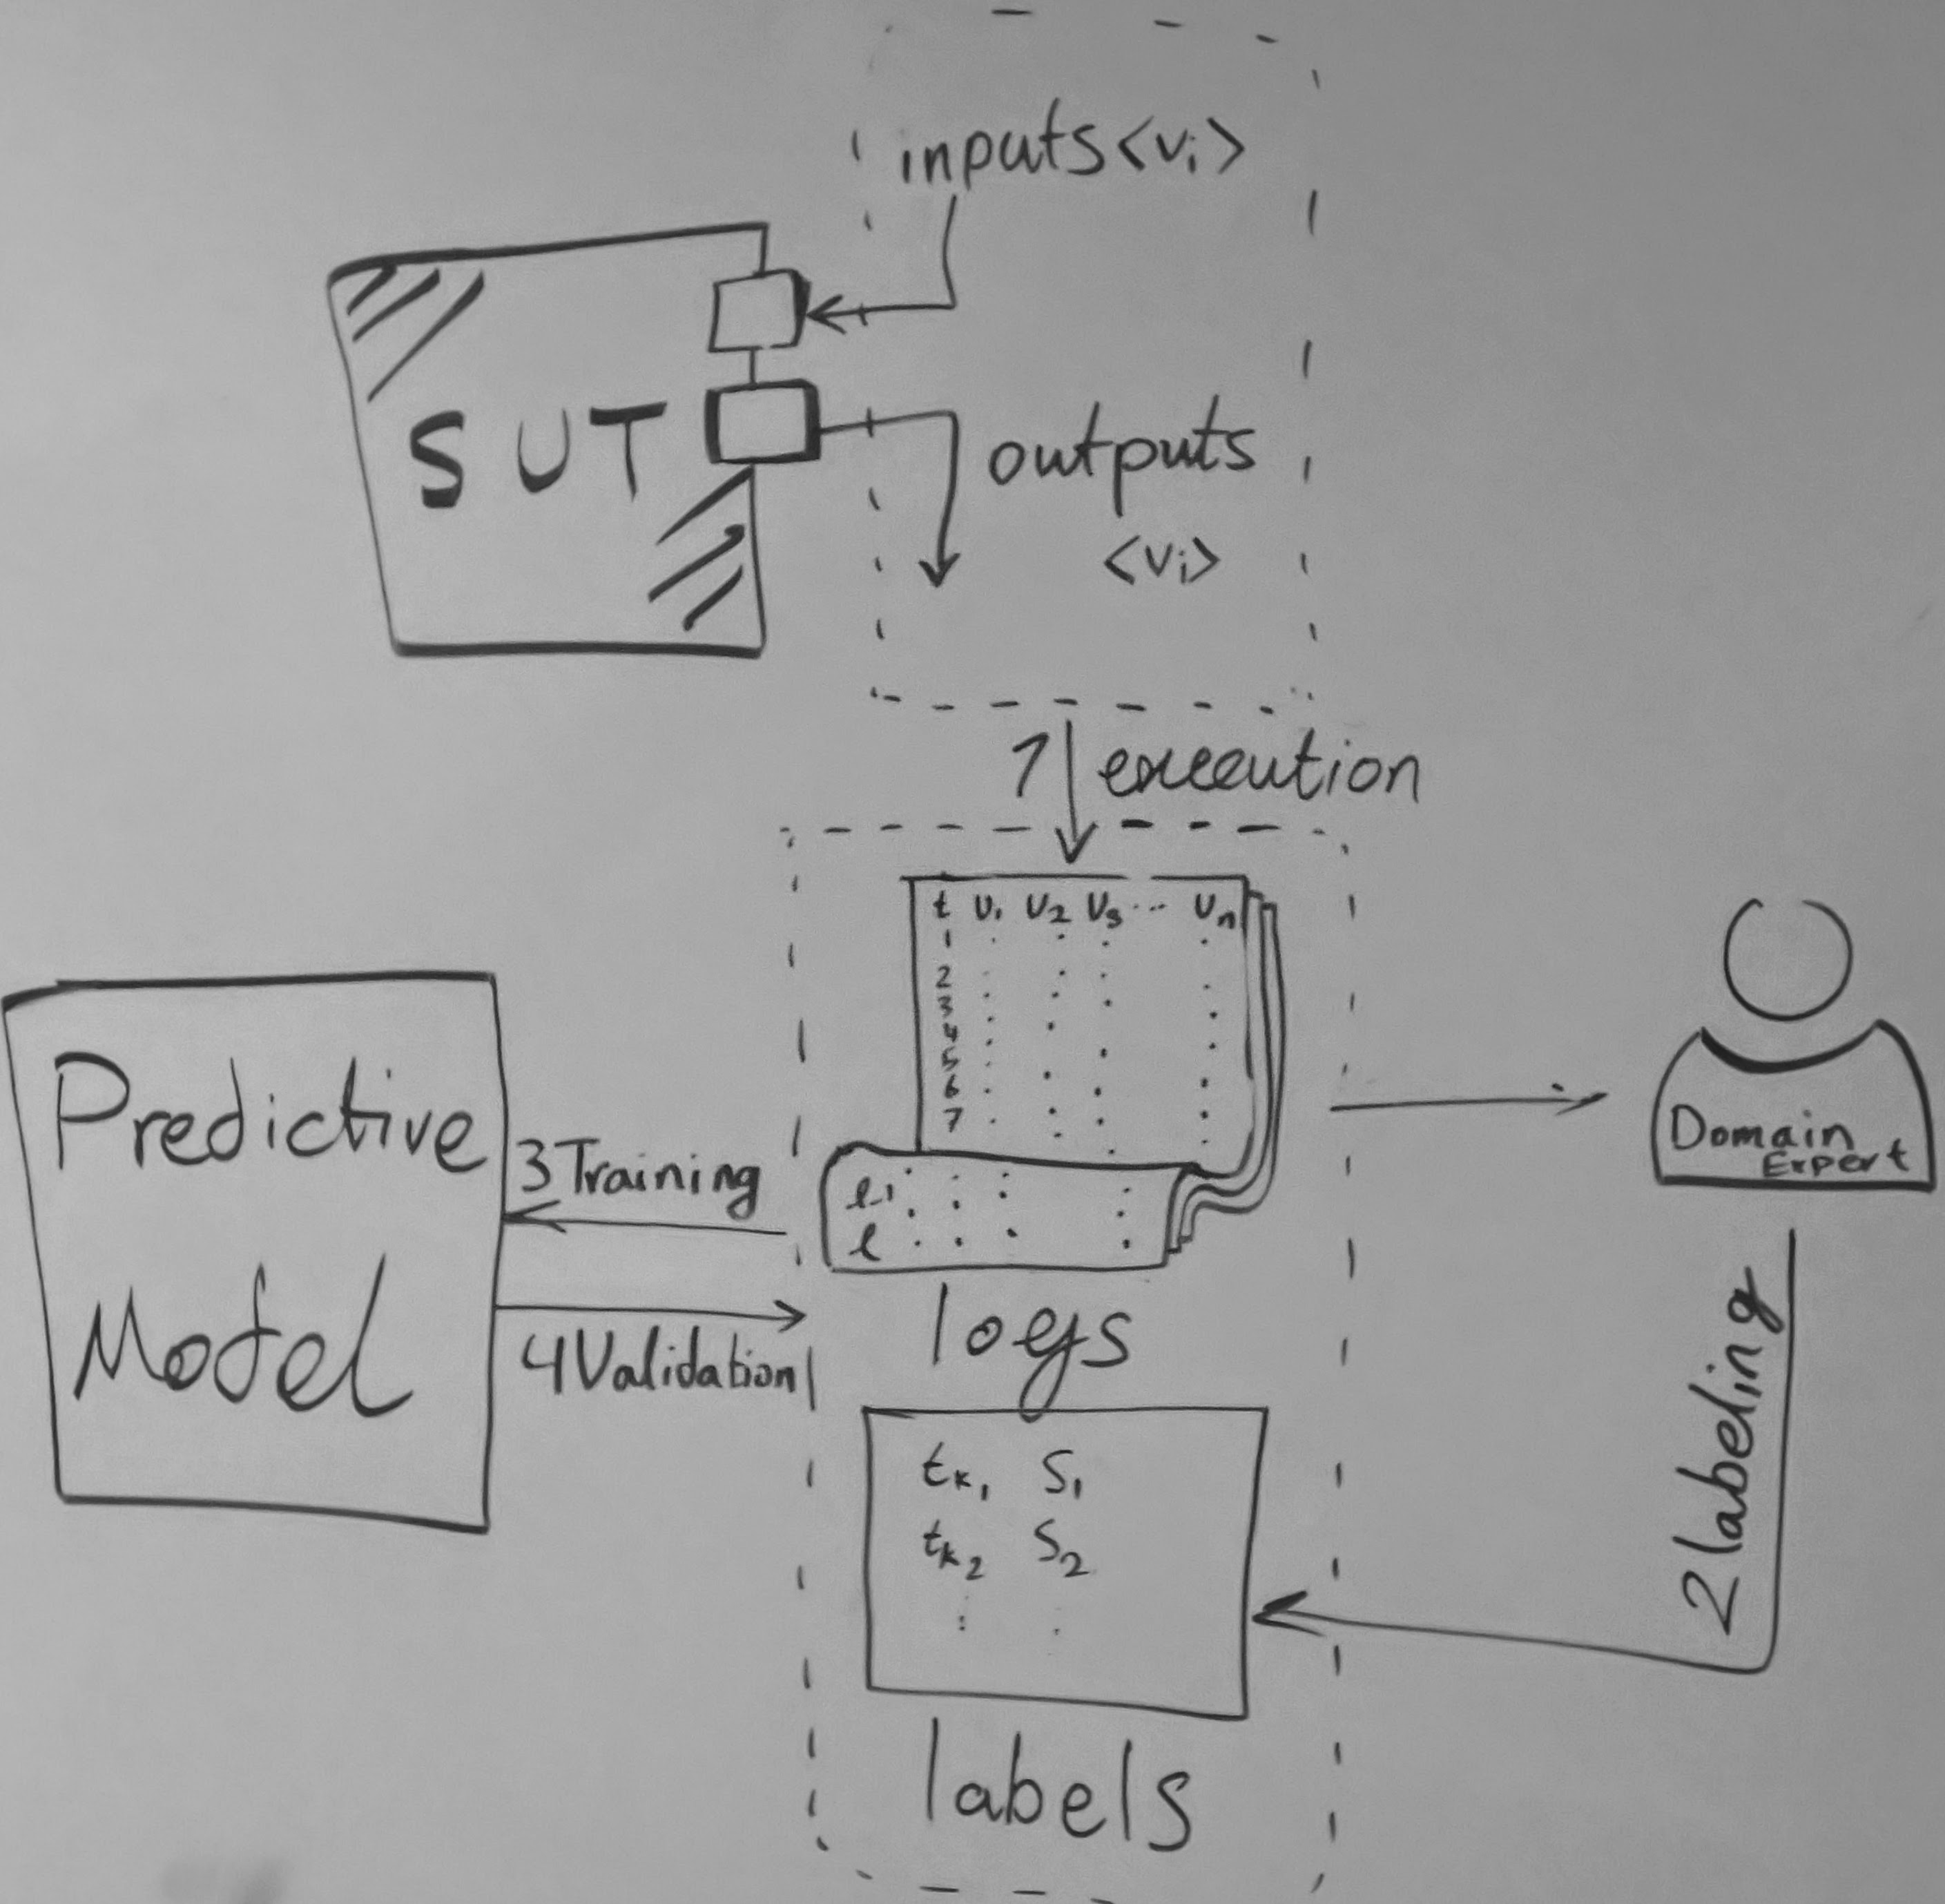
\includegraphics[width=\columnwidth]{Sections/process_diagram.jpg}
    \caption{This diagram shows a big picture of how this technique is applied. The object system is treated as a black-box where we can only read its input and output values. In the first step the system is executed and multiple logs of the input/output values are recorded. Second, a domain expert labels the logs indicating the time stamps where the system's internal state has changed as well as the new state that it went in. In third and fourth steps, as it is typical in machine learning based solutions these data and labels are used for training and validating a machine learning model.}
    \label{fig:process_diagram}
\end{figure}

Combining all, each training instance will be the tuple $(T_k, CP_k)$.

\subsection{Proposed Machine Learning Model}
\subsubsection{Inputs and Labels} \label{data_set_properties}


Since TensorFlow requires all the data to have the same shape, the shorter $T_k$s should be zero-padded to length ,$L = max\{l_k\}$.
Therefore in the end the input to the model will be $T_k$s that are rearranged to form a tensor of shape $n \times L$ along with a padding mask. Padding mask is used to prevent the added zero values having a negative effect on the model's performance. It tells the model where the tail starts so the model can ignore all the zeros from there on.

The true labels ($O$, also called labels in ML literature) is a vector of length $L$ (after padding) where each element $\o_t$ holds the one-hot encoded state at time $t$. It can be determined easily by consulting set $CP_k$ (definition \eqref{eq:change_point}) as defined in \eqref{eq:output}.
\begin{equation} \label{eq:output}
\begin{split}
O = \langle  \forall t \in \mathbb{N}_L : s_i | 
            &{} (t_{s_i}, s_i) \in CP_k \land  \\
            & t_{s_i} = max\{t_{s_j} | (t_{s_j}, s_j) \in CP_k \land t_{s_j}\leq t\} \rangle
\end{split}
\end{equation}
The tensor shapes mentioned here ignore the batch size dimension.

The goal is to find a model $\mathcal{F}(T^p, \mu) \colon \mathbb{R}^{L\times n}\times\mathbb{R}^L\to\mathbb{R}^{L}$ that best approximates the system's behaviour in terms of estimating its internal state given the $n$ time series containing sampled in/out values of the system all zero padded to length $L$.

\begin{equation}\label{eq:model_as_function}
\begin{split}
    \hat{O} = \langle \hat{o}_i \in S \rangle^L_{i=1} {}&{}= \mathcal{F}\left(\left[ {V^p_1}^\intercal \: {V^p_2}^\intercal \; \ldots \; {V^p_n}^\intercal \right], \langle {mask}_j \rangle^L_{j=1}\right) \\
    \langle {mask}_j \rangle^l_{j=1} {}&{}= 1  \\
    \langle {mask}_j \rangle^L_{j=l+1} {}&{}= 0 \\
    V^p_i {}&{}= \left[V_i \quad \vec{0}_{L-l}\right]
\end{split}
\end{equation}

In \eqref{eq:model_as_function} $l$ denotes the length of the input before padding; for the $k$th training data ($T_k$) it is the same as $l_k$. The superscript $p$ for input variables emphasises on the post-padding applied on the original variables which is also shown in the equation.

\subsubsection{Architecture}


We used 4 convolutional layers with 64 filters and kernel sizes of 3, 5, 10, 15 respectively.
%with max pooling layers of size 2 in between. 
Their output is fed into two recurrent layers with 128 and 96 cells each which are then fed into two fully connected layers of size 96 and $N_s$ units. This last layer has a `softmax' activation function.
%This layer's output is fed to an upsampling layer to match the length of the output to length of the labels vector.  
This architecture forms a CNN-RNN hybrid neural network. \cite{Wang2017}


\subsubsection{Architecture Justification}
As mentioned in \ref{changes_in_inputs} since what matters more are the changes rather than the absolute values, applying a derivation operation (or more generally a gradient) is necessary at some point in the processing. 
Farid and Simoncelli enumerated some discrete derivation kernels \cite{Farid2004}, but to have a more generalized notion of discrete derivatives we used convolutional layers in a neural network model. 

Applying convolutional filters on signals is pretty much a standard process in signal processing projects that take deep learning approaches.  \cite{morales2016deep, zeng2014convolutional, yang2015deep} Since convolutional layers on time series basically provide a way to perform calculations on the signal readings spanning a window of time they are effective in capturing features involving temporal relations and invariants in the signals. \cite{wang2017time} 
Using convolutional layers instead of predefined kernels allows the model to learn which subset of possible correlations (which can involve two or more variables) it needs to focus on. This type of flexibility has another benefit as well. It helps the model to be more resilient to time lag between noticing a deviation in input signals and the reaction that will appear in the output signals. This time lag can be caused by a number of reasons including: physical limitations, sampling resolution, tuning of the controller, or design choices in the system.

The recurrent layers introduce an element of `memory' allowing them to capture long-term temporal dependencies which is quite useful in our use case. \cite{Che2018} RNNs have shown promising results in various deep learning for time series tasks such as prediction and classification. \cite{wang2017time, murad2017deep, yang2015deep, Ordonez2016}

This architecture is in part inspired by auto-encoder architectures proposed for image segmentation task. (Add citations and more explanation)